\documentclass[12pt, notitlepage]{article}

\usepackage{amssymb,amsmath,mathabx,hyperref,graphicx,multirow, array, subfigure} 

\usepackage{mdwlist}

\newenvironment{packed_list}{
\begin{itemize*}
\setlength{\itemsep}{0pt}
\setlength{\parskip}{0pt}
\setlength{\parsep}{0pt}
\setlength{\headsep}{0pt}
\setlength{\topskip}{0pt}
\setlength{\topmargin}{0pt}
\setlength{\topsep}{0pt}
\setlength{\partopsep}{0pt}
}{\end{itemize*}}

\begin{document}

\title{CSE 6730 Project Report:\\Parallel Molecular Dynamics Simulation}
\author{Mary Benage, Andrew Champion,\\Zhejiang Dong, Mohan Rajendran\\
  \\
 Georgia Institute of Technology}
\date{April 27, 2012}
\maketitle

\section*{Introduction}

Molecular dynamics simulations allow researchers to investigate phenomena emergent in systems at the molecular scale, such as protein assembly and formation of hydrodynamic flows. The goal of this project is to implement a cluster-parallelized molecular dynamics simulation (PMDS) for periodic systems on the order of thousands of entities. To meet this goal, this project's objectives are to implement a simulation of Lennard-Jones potentials \cite{jones1924determination} and bonds between atoms and parallelize this simulation with MPI by distributing atoms and decomposed blocks of the force matrix to nodes in the system. We used only the short-range force models and ignore the Coulomb forces to limit the computational effort and to meet the criteria of \cite{plimpton1995fast} to parallelize the algorithm. To validate this implementation, a model of lipid-like entities in a solution was simulated and the results compared with theoretical expectations and simulation outcomes from the LAMMPS Molecular Dynamics Simulator \cite{plimpton1995fast, lammps}.

\section*{Background}

Molecular dynamics simulations are used to compute equilibrium and transport properties of interacting molecules that obey the laws of classical mechanics. A typical  simulation has a timestep around femptoseconds and therefore tens, hundreds or thousands of timesteps are needed \cite{plimpton1995fast}. The first molecular dynamic paper was in 1956 by Alder and Wainwright at Livermore National Laboratory. Molecular dynamics simulations have since been used essentially as real experiments aimed at better understanding properties of materials such as liquids and solids. The approach for these numerical experiments are as follows: prepare the sample with the proper structure, equilibrate the system by solving Newton's equations of motion for the N atoms until there is no change, then perform the experiment \cite{frenkel2002understanding}.

The individual force equations for each atom are derived from the potential energy functions, such as the Lennard-Jones potential used for calculating van der Waals forces. MD simulations extensively only solve the short-range forces -- bonded forces and van der Waals -- and ignore the long-range Coulombic forces \cite{plimpton1995fast, lammps}. MD simulations typically have periodic boundary conditions and a cutoff distance for the distance between each pair of atoms, i and j. The cutoff distance is used to limit the number of calculations, thus if the distance between two atoms is greater than the cutoff distance, their force is not calculated. The distance between two atoms is used to solve the Lennard-Jones potential (or other potentials) and update the forces for each atom \cite{frenkel2002understanding}. The most computationally intensive part of MD simulations is the computation of the forces. There are two common methods to reduce computation by limiting the number of times the algorithm has to check that atoms are within the cutoff distance: the neighbor list and link-cell method or a combination of the two \cite{plimpton1995fast, lammps}. Once the forces are determined, individual atoms' motion is found by integrating Newton's equation of motion, commonly using the Verlet algorithm \cite{frenkel2002understanding}.

Molecular dynamics are considered inherently parallel since the force and position updates can be done simultaneously. We will follow the methods proposed by \cite{plimpton1995fast} to parallelize. The two basic assumptions for this method are that the forces are limited in range or are only short-range forces, and the atoms can undergo large displacements. The three basic methods proposed for parallelization are either atom decomposition, force decomposition, or spatial decomposition. Atom decomposition assigns a subset of atoms to each processor and that processor is responsible for calculating the total forces on each atom and updating the velocity and positions of it's atoms. Force decomposition assigns each processor with a fixed set of atom pairs that it is responsible for calculating the force. There is then a fold operation and each processor is then responsible for updating the position and velocity of a subset of atoms (it is the same as in the atom decomposition). Lastly, spatial decomposition assigns a fixed space to each processor. At each timestep, the processor calculates force and updates position and velocity for each atom in its associated space. In this decomposition, the atoms will move among processors. In summary, the atom and force decompositions are analogous to a Lagrangian frame of reference and spatial decomposition is analogous to an Eulerian frame of reference \cite {plimpton1995fast,shaw2005a}. 


\subsection*{Neighbour List}
Due to the fact that the intermolecular forces considered are short-range, we do  not need to consider all the pairs of atoms for the purpose of force calculation. A na\"ive method which goes through all the pairs of particles assigned to a processor would have a time complexity $O(N^2)$. Thus, the concept of Verlet neighbour list presented in \cite{verlet1967} is used. This concept uses an array for each particle in each processor to maintain the list of local particles within the cut-off radius $r_c$ plus a small distance $r_s$ called skin distance.

\begin{figure}[!]
\begin{center}
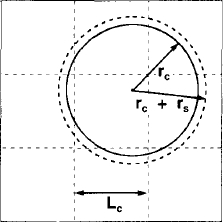
\includegraphics[width=2.5in]{figures/neigh_list.jpg}
\caption{Illustration of relationship between cut-off radius $r_c$, skin distance $r_s$, and cell length $L_c$.}
\label{fig:neighbor}
\end{center}
\end{figure}

When particle interactions are calculated, only the particles in the neighbour list are considered. This saves computation time by removing the need to look for all the particles in the system. Further, the skin radius gives leeway by tracking particles slightly beyond of the cut-off radius. This means that the neighbour list need not be updated every timestep.

Further, the solution domain may be divided into cells of length $L_c\leq r_c+r_s$ and each cell can have its own linked list of atoms lying within that cell. When a neighbour list is built, the program need not check all the cells but only 9 cells forming the square around the atom in consideration. This reduces the computation time further. However, if the number of particles tracked by each processor is small, there is no need to create the cell list.

\section*{Serial Simulation}
The following simulation procedure has been adapted from \cite{lammps} and gives a general procedure and formulas involved in the solution procedure. Please refer to Figures \ref{fig:flow_init}-\ref{fig:flow_integration} for a flow chart of the algorithms used.
\begin{enumerate}
  \item Set all the atoms in their locations by reading from an input file from LAMMPS. \\
  See \texttt{parser.f90}, \texttt{in.micelle}, and \texttt{data.micelle}.
  \begin{enumerate}
    \item 1200 atoms - 750 water(1), 150 head(2), 150 tail1(3), 150 tail2(4)
    \item 300 bonds
    \item Bounding box (0,0) to (35.85686,35.85686)
  \end{enumerate}
  \item Let system attain thermal equilibrium \\
  See \texttt{parser.f90}, \texttt{initial.f90}, \texttt{pmds.f90}, \texttt{force\_soft.f90} (or \texttt{force\_\-soft\_neighbor.f90}, \texttt{neighbor.f90} for use of neighbor list), \texttt{integrate.f90}, \texttt{normalize\_vel.f90}, and \texttt{in.micelle}. \\
(Note: parameters are defined below in equations used)
  \begin{enumerate}
    \item Set special bonds to fene which sets LJ interaction with parameters 0, 1.0 and 1.0
    \item Set pair style between all atoms as soft interactions with parameters 0, 1.2246
    \item Set bond style between atoms to be harmonic with parameters 50.0, 0.75
    \item Set initial velocity with uniform distribution for temperature 0.45
    \item Set integration conditions(fix)
    \begin{enumerate}
      \item Set NVE(Number, Volume, Energy) conservation integration 
      \item Update temperature to 0.45 every 100 time steps by rescaling velocity
      \item Set soft interaction constant A to ramp from 1 to 20 as time proceeds
    \end{enumerate}
    \item Run for 1000 timesteps
  \end{enumerate}
  \item Actual development of micelle layer
  \begin{enumerate}
    \item Remove soft interactions\\
Set interaction style to Lennard Jones with cut-off\\
\begin{tabular}{ | c | c | r | r | r | }
\hline
atom1 & atom2 & $\epsilon$ & $\sigma$ & $r_c$ \\
\hline
water & water &1.0 &1.0 &2.5\\
head & head &1.0 &1.0 &2.5\\
water & head &1.0 &1.0 &2.5\\
tail 1 & tail 1 &1.0 &0.75 & 2.5\\
tail 2 & tail 2 &1.0 &0.50 &2.5\\
tail 1 & tail 2 &1.0 &0.67 &2.5\\
water & tail 1 &1.0 &1.0 &1.12246\\
water & tail 2 &1.0 &1.0 &1.12246\\
head & tail 1 &1.0 &0.88 &1.12246\\
head & tail 2 &1.0 &0.75 &1.12246\\
\hline
\end{tabular}
    \item Run for 60000 time steps
    \end{enumerate}
\end{enumerate}

The serial algorithm for the force computation and integration is below. For the serial version we took advantage of Newton�s Third Law, thus decreasing the force computation cost in half. 

\subsection*{Force}

See \texttt{force.f90} and \texttt{soft\_force.f90} (or \texttt{force\_neighbor.f90}, \texttt{force\_soft\_neighbor.f90} and \texttt{neighbour.f90})

\begin{itemize}
\item Loop through each atom to calculate the distance between two atoms (or loop through neighbor list)
  \begin{itemize}
    \item 1st loop through particle $i = 1$ to $N_{atom} -1$
    \item 2nd loop through particle $j = i+1$ to $N_{atom}$
      \begin{itemize}
        \item Calculate distance (X and Y) between two particles based on their positions.
        \item e.g. Distance $= X(i)-X(j)$
      \end{itemize}
    \item apply periodic boundary conditions to both $D_X$ \& $D_Y$
      \begin{itemize}
        \item $D_X=D_X-\texttt{box}*\texttt{nint}(D_X/\texttt{box})$
      \end{itemize}
    \item Calculate $R^2 = D_X^2 + D_Y^2$
  \end{itemize}
\item Determine the atom type for $i$ \& $j$ using the array atom type (called AT in code)
\item Use the atom types to query matrix of parameters needed to calculate force
  \begin{itemize}
    \item Lennard Jones: cut off radius, sigma, epsilon (See 3.b. above)
    \item Soft: cut off radius, energy (See 2.b. above)
    \item Harmonic Bonds: energy/distance$^2$ , equilibrium bond distance (See 2.c. above)
  \end{itemize}
\item Calculate the Nonbonded Forces using either Soft for initialization or Lennard-Jones for the Simulation Run. 
  \begin{itemize}
    \item Lennard Jones: $F = - \frac{48\epsilon r}{r^2 \sigma}\left(\frac{\sigma}{r}\right)^6\left[\left(\frac{\sigma}{r}\right)^6 - 0.5\right] dx \text{ (or $dy$)}$
    \item Soft: $F = -A\left[\frac{\pi}{r_c}\sin\left(\frac{\pi r}{r_c}\right)\right] dx \text{ (or $dy$)}$
    \item Update total forces on atoms using Newton�s Third Law:
    \begin{align*}
    F_x(i) &= F_x(i) + FD_X \\
    F_y(j) &= F_y(j) - FD_Y
    \end{align*}
  \end{itemize}
\item Loop through the atom bonded list to calculate the bond forces
  \begin{itemize}
    \item Harmonic Bonds: $F = -2k(r - r_o) dx \text{ (or $dy$)}$
    \item Update total forces on atoms using Newton�s Third Law:
    \begin{align*}
    F_x(i) &= F_x(i) + FD_X \\
    F_y(j) &= F_y(j) - FD_Y
    \end{align*}
  \end{itemize}
\item End when have looped through all the atoms. 
\end{itemize}


\subsection*{Integration}
See \texttt{integrate.f90} and \texttt{normalize\_vel.f90}
\begin{itemize}
\item Loop through each particle
  \begin{itemize}
    \item Calculate predicted position\\
	$x'(t+\Delta t)=2x(t)-x(t-t\Delta )+\frac{F(t)}{\Delta t^22}$
    \item Calculate predicted velocity\\
	$v'(t)=\frac{x'(t+\Delta t)-x(t- \Delta t)}{2\Delta t}$
    \item Sum up kinetic energy \\
	$U_{kin}=U_{kin}+\frac{v_x^2+v_y^2}{2}$
  \end{itemize}
\item At every Estep, rescale to ensure desired temperature
  \begin{itemize}
    \item Calculate velocity scaling\\
	$scale = \sqrt{\frac{(2N-2)*T_{desired}}{U_{kin}}}$
  \end{itemize}
\item Loop through each particle
  \begin{itemize}
    \item Find actual velocity\\
$v(t)=scale*v'(t)$
    \item Find actual position\\
$x(t+ \Delta t)=x(t- \Delta t)+v(t)*2\Delta t$
    \item Increment timestep\\
$x(t- \Delta t)=x(t)$
$x(t)=x(t+ \Delta t)$
    \item Make sure all particles end up inside box
  \end{itemize}
\end{itemize}

\subsection*{Neighbor List}
See \texttt{neighbour.f90}

\begin{itemize}
\item Set up cells
  \begin{itemize}
    \item Set the cell width to be equal to the maximum of cut-off radius + skin radius
    \item Increase the cell width slightly so that the cell size divides the box size evenly
    \item Calculate number of cell in each direction(no. of cells = numcell$^2$)
  \end{itemize}
\item Bin atoms via a linked list
  \begin{itemize}
    \item Loop through all cells
      \begin{itemize}
        \item Set head of linked list(cellnum) = 0
      \end{itemize}
    \item Loop through atoms
      \begin{itemize}
        \item Calculate the i and j index of the cell where the current atom belongs to
        \item Using i and j calculate the actual cellID (j*numcell+i)
        \item Set LL(atomID) = head(cellID)
        \item head(cellID) = atomID
        \begin{itemize}
          \item This method stores numbers in an array of size equal to the number of atoms. To retrieve the atoms in a given cell, we just go to LL(head(cellID)) and loop backwards to LL(LL(head(cellID))) and so on till LL(atom) = 0
        \end{itemize}
    \end{itemize}
  \end{itemize}
\item Set up neighbour list
  \begin{itemize}
    \item Loop through all atoms
      \begin{itemize}
        \item Set number of entries in current atom�s neighbour list to zero
        \item Calculate the cell that the current atom belongs to
        \item Offset the cell by -1,0 and 1 in each direction
          \begin{itemize}
            \item At each of these cells, loop through the atoms in the cell
If distance between the two atoms is less than $r_{skin}+r_{cutoff}$, add to the neighbour list of whichever atom has the higher atomID
          \end{itemize}
      \end{itemize}
  \end{itemize}
\end{itemize}

\subsection*{Equations Used}

The following equations are used in the simulation, where $E$ is potential energy and $F$ is force.
\begin{itemize}
\item Lennard-Jones interaction
  \begin{align*}
  E &= 4\left[\left(\frac{\sigma}{r}\right)^{12}-\left(\frac{\sigma}{r}\right)^{6}\right] \text{ for } r<r_c \\
  F &= - \frac{48\epsilon r}{r^2 \sigma}\left(\frac{\sigma}{r}\right)^6\left[\left(\frac{\sigma}{r}\right)^6 - 0.5\right] dx \text{ (or $dy$)}
  \end{align*}
  Parameters: $\epsilon$, $\sigma$, $r_c$
  
\item Soft interaction
  \begin{align*}
  E &= A\left[1 + \cos\left(\frac{\pi r}{r_c}\right)\right] \text{ for } r < r_c \\
  F &= -A\left[\frac{\pi}{r_c}\sin\left(\frac{\pi r}{r_c}\right)\right] dx \text{ (or $dy$)}
  \end{align*}
  Parameters: $A$, $r_c$
  
\item Harmonic bonds
  \begin{align*}
  E &= k(r - r_o)^2 \\
  F &= -2k(r - r_o)
  \end{align*}
  Parameters: $k$, $r_o$
  
\item Temperature-velocity formula for 2D cases
  \begin{align*}
  \frac{1}{2}m < v^2 > =& kT
  \end{align*}
  
\item Verlet velocity integration (NVE)
  \begin{align*}
  x(t + \Delta t) &= x(t) + v(t) \Delta t + \frac{F(t)}{2m}\Delta t^2\\
  v(t + \Delta t) &= v(t) + \frac{F(t) + F(t + \Delta t)}{2m}\Delta t
  \end{align*}
  
\item Kinetic energy
  \begin{align*}
  U_{kin} &= \sum \frac{1}{2}m(v_x^2 + v_y^2)
  \end{align*}
  
\item Temperature
  \begin{align*}
  T &= \frac{U_{kin}}{2N-2}
  \end{align*}
  
\item Pressure
  \begin{align*}
  P &= \frac{NT}{V} + \frac{1}{6V} \sum r_{ij}\cdot f_{ij}
  \end{align*}

\end{itemize}

\section*{Parallelization Process}

The parallelization process that was used is adopted from \cite {plimpton1995fast}. The method involves the use of a distributed memory system to run the simulation procedure. For simplicity, atom and processor numbers are chosen so N/P atoms can be assigned to each processor. The parallelization was implemented using a procedure called atom decomposition, where the atoms are assigned to processors at the start of the simulation and the processor is responsible for updating the position of its assigned atom through the time integration of Newton�s equations of motion. We implemented two forms of the atom decomposition, called A1 or A2. A1 calculates the total force on each atom and does not take advantage of Newton's Third Law. The A2 implementation takes advantage of Newton's Third Law and decreases the computation cost of the forces in half as compared to A1. There are added communication costs for A2, since while A1 requires only a single collective operation per timestep to exchange atom positions, A2 must exchange forces and pressures.

The algorithm for atom decomposition 1 per timestep and per processor is as follows:
\begin{enumerate}
\item Send and receive the particle positions to and from all the processors (fold operation).
\item Determine which forces to be computed using the neighbor lists.
\item Compute the total force for each atom
\item Do time integration of Newton's equations of motion to update assigned atom velocity and position. 
\end{enumerate}

\subsubsection*{Atom Decomposition 2}
This approach takes advantage of Newton�s 3rd Law, $F_{ij} = - F_{ji}$, where it computes the force between a pair of atoms once and not twice. A processor is responsible for calculating the force that $N/P$ atoms have between them and the rest of atoms. And, it calculates the force between a pair of atom when their ID satisfies: $i<j$ and $i+j$ is even, or $i>j$ and $i+j$ is odd. Figure \ref{fig:a2decomp} shows an 8 atoms 2 processors example, processor 1 is responsible for the force calculations for lattice marked in red and processor 2 is responsible for those in blue. They will compute the force only for the lattice marked with a cross sign. And, as shown in the right matrix of Figure \ref{fig:a2decomp}, if we fold the matrix along the red line, the lattice will cover lower triangle of the matrix without overlapping, which indicates the property that the force between all the pair have been covered once and only once. After finishing the force calculation, each processor does a \texttt{MPI\_ALLREDUCE} operation to compute the total force acting on each atom, and then they update the position for N/P atoms with performing an \texttt{MPI\_ALLGATHER} operation to collect the updated position for all atoms.

\subsection*{Performance Evaluation}

The performance of our program is evaluated over time consumption, which was obtained from 1200 atoms, 10,000 time steps simulation runs. As shown in Figure \ref{fig:strongscale}, with neighbor list optimization we obtained over 6 times the speedup compared to the case without any optimization. The best case atom decomposition can lead to another 30\% speed up on top of neighbor list implementation due to utilizing Newton�s third law and the elimination of redundant calculations. Atom decomposition 2 has slightly better performance than atom decomposition 1. An interesting observation is that the  introduction of more processors increased the time consumption. One possible reason for this phenomenon is when the problem scale is relatively small, the time consumed during communication can overwhelm the speedup gain by introducing more computational power. 

To evaluate the weak scaling performance of the serial, A1 and A2 implementations, a generator was written to create micelle datasets for arbitrary numbers of atoms. In these generated datasets, the atoms are initialized on a grid of the same scale as the original dataset, only the bounds of the simulation and extent of the grid are varied to fit the requested number of atoms. Molecules are randomly initialized on atoms in the grid as in the original dataset, maintaining the same ratio of molecules to atoms as the original dataset. As shown in Figure \ref{fig:weakscale}, with these generated datasets, the runtime of each of the implementations was averaged across 5 trials for process counts of $2^i$ for $i \in [0, 4]$ (or 1 process for the serial implementation). Since weak scaling considers performance as the problem size per process is held constant, this corresponds to problem sizes between 1200 and 19,200 atoms. As expected, the serial implementation has the longest runtime. Though it requires somewhat less communication than A2, A1 is slower than A2 since it requires twice the amount of computation. 

\section*{Validation}

LAMMPS \cite{lammps} is a widely used and well tested molecular simulation tool. We validated the following data in our simulation against that obtained by running LAMMPS. We ran 10 runs for our code and 10 for LAMMPS and each was started with a different random seed for initial velocity. We then took the average of the 10 runs and compared the following values:
\begin{enumerate}
\item Total Energy over time
\item Final velocity distribution
\item Pressure over time
\end{enumerate}
As shown in Figures \ref{fig:valvel}-\ref{fig:valtot}, with same trend and a acceptable deviation, our simulation result agree with that of LAMMPS simulation.

\newpage

\bibliographystyle{plain}
\bibliography{pmds}

\newpage

\begin{figure}
\begin{center}
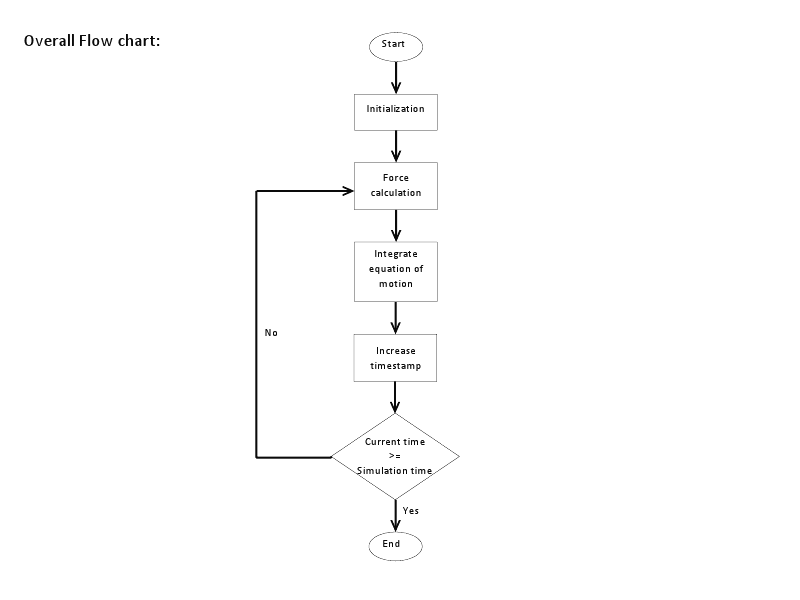
\includegraphics[width=8in]{figures/flow_overall.png}
\caption{Flow chart of the main simulation loop.}
\label{fig:flow_overall}
\end{center}
\end{figure}

\newpage

\begin{figure}
\begin{center}
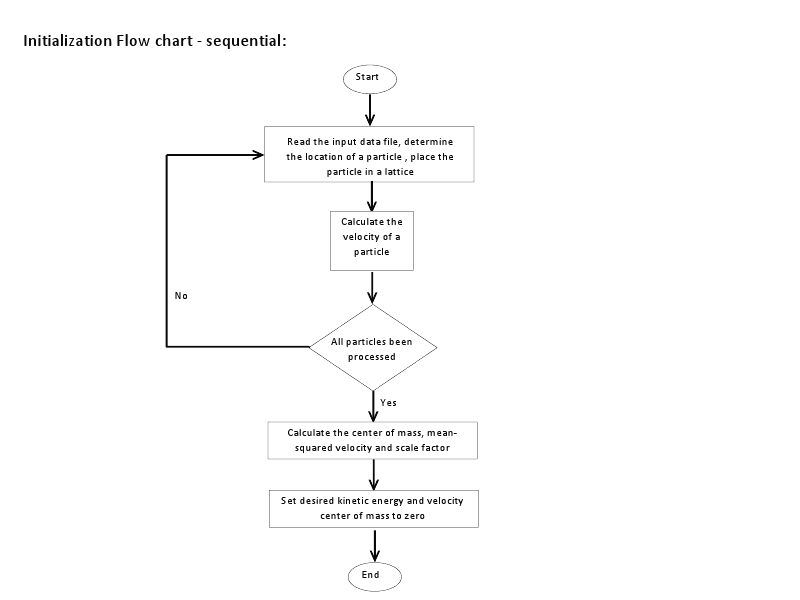
\includegraphics[width=8in]{figures/flow_init.png}
\caption{Flow chart of the model initialization.}
\label{fig:flow_init}
\end{center}
\end{figure}

\newpage

\begin{figure}
\begin{center}
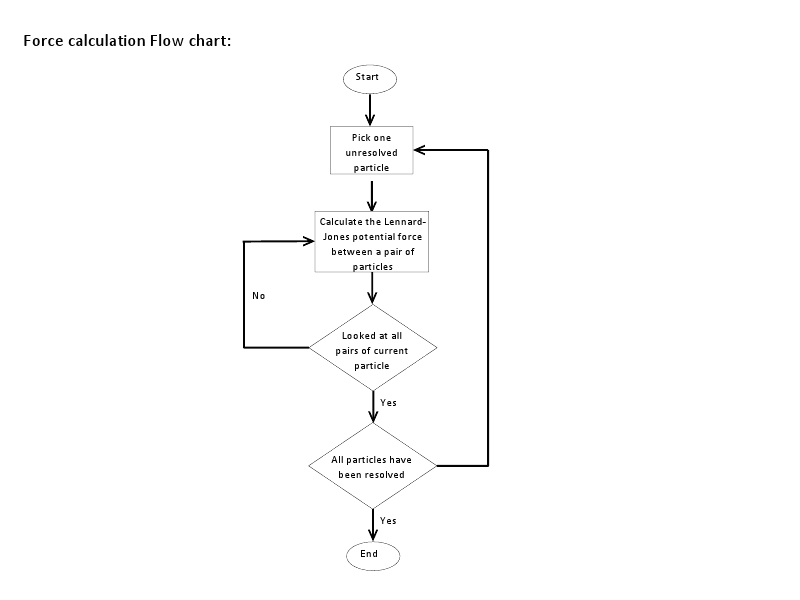
\includegraphics[width=8in]{figures/flow_force.png}
\caption{Flow chart of sequential force calculation.}
\label{fig:flow_force}
\end{center}
\end{figure}

\newpage

\begin{figure}
\begin{center}
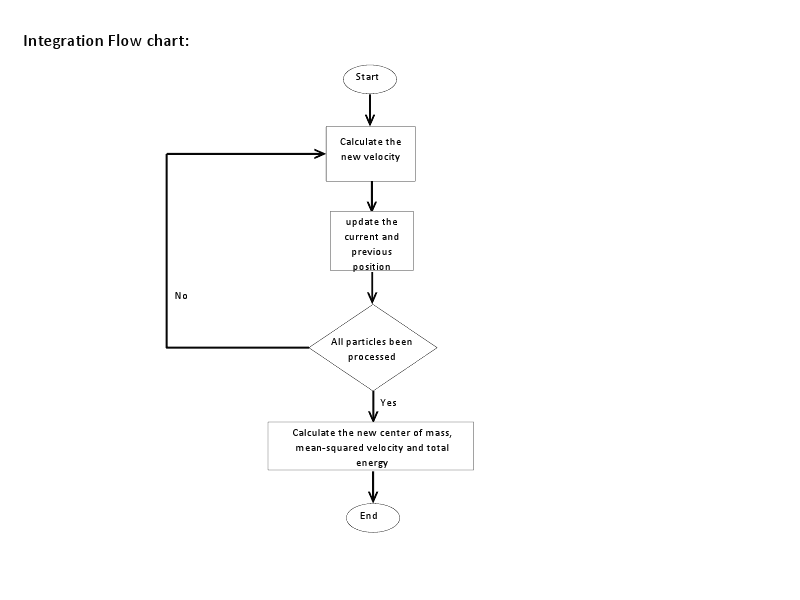
\includegraphics[width=8in]{figures/flow_integration.png}
\caption{Flow chart of velocity integration.}
\label{fig:flow_integration}
\end{center}
\end{figure}

\begin{figure}
\begin{center}
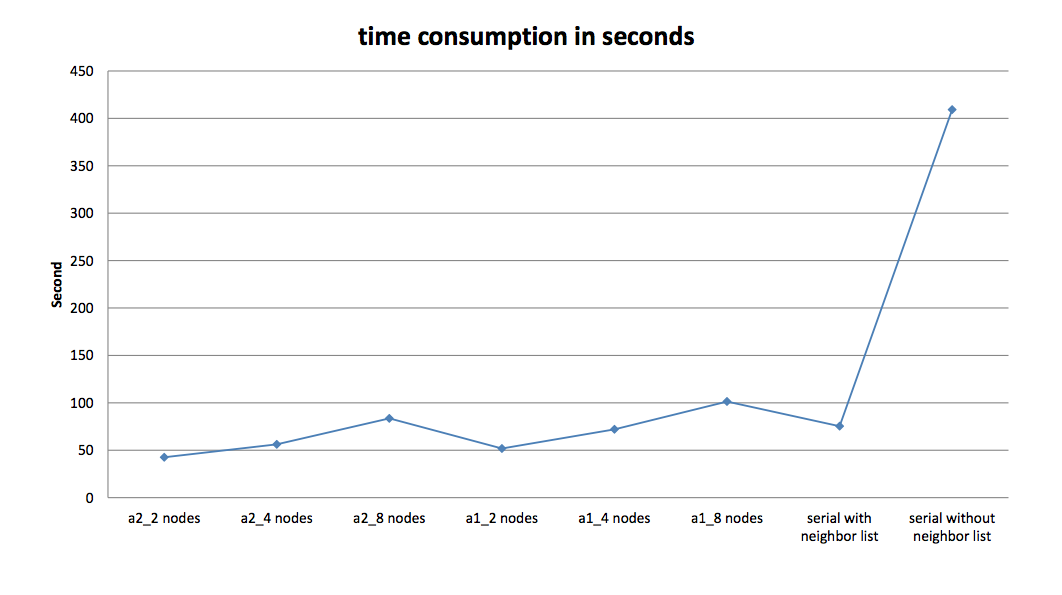
\includegraphics[width=6in]{figures/strongscale.png}
\caption{Strong scaling performance for small problem size of the three implementations.}
\label{fig:strongscale}
\end{center}
\end{figure}

\begin{figure}
\begin{center}
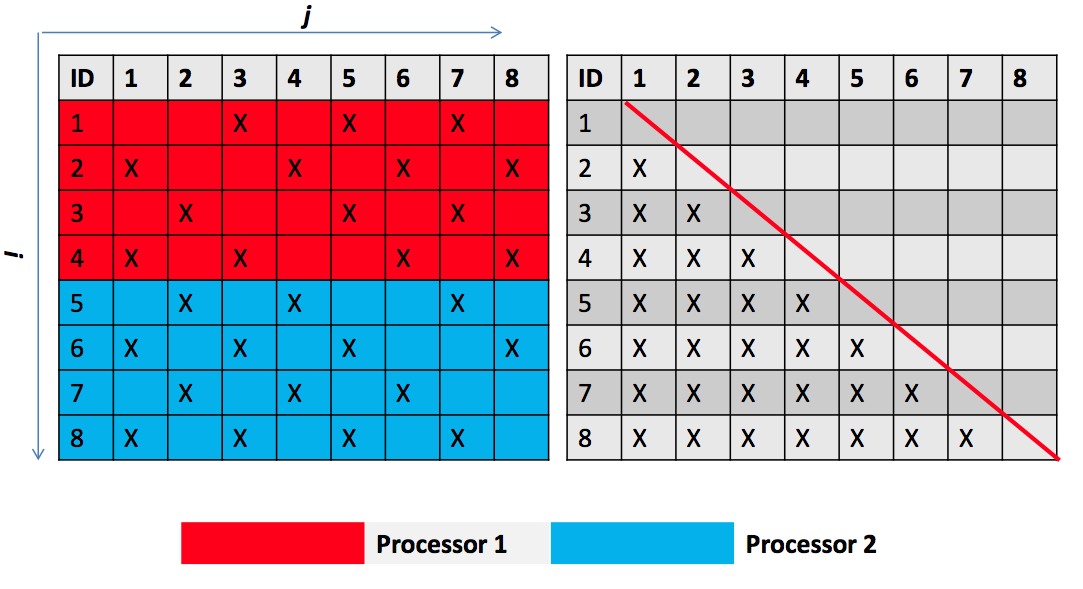
\includegraphics[width=6in]{figures/a2decomp.png}
\caption{Atom decomposition 2 of force matrix calculation. Entries marked with `X' are calculated, while others are skipped. The right matrix shows that if folded along the diagonal, the left matrix is triangular.}
\label{fig:a2decomp}
\end{center}
\end{figure}

\begin{figure}
\begin{center}
\subfigure[Our Implementation]{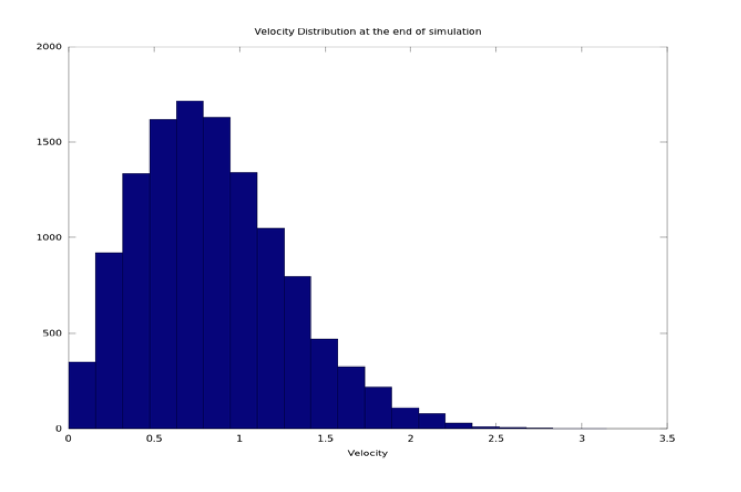
\includegraphics[width=5in]{figures/vel_ours.png}}
\subfigure[LAMMPS]{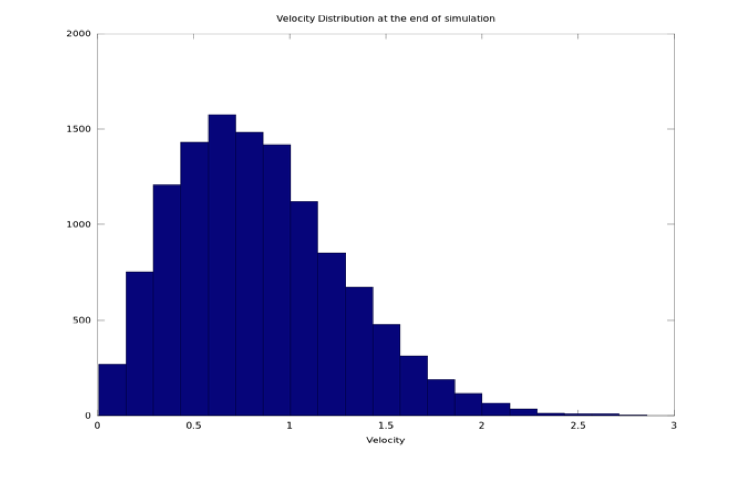
\includegraphics[width=5in]{figures/vel_lammps.png}}
\caption{Distribution of velocity at the end of simulation averaged over 10 trials.}
\label{fig:valvel}
\end{center}
\end{figure}

\begin{figure}
\begin{center}
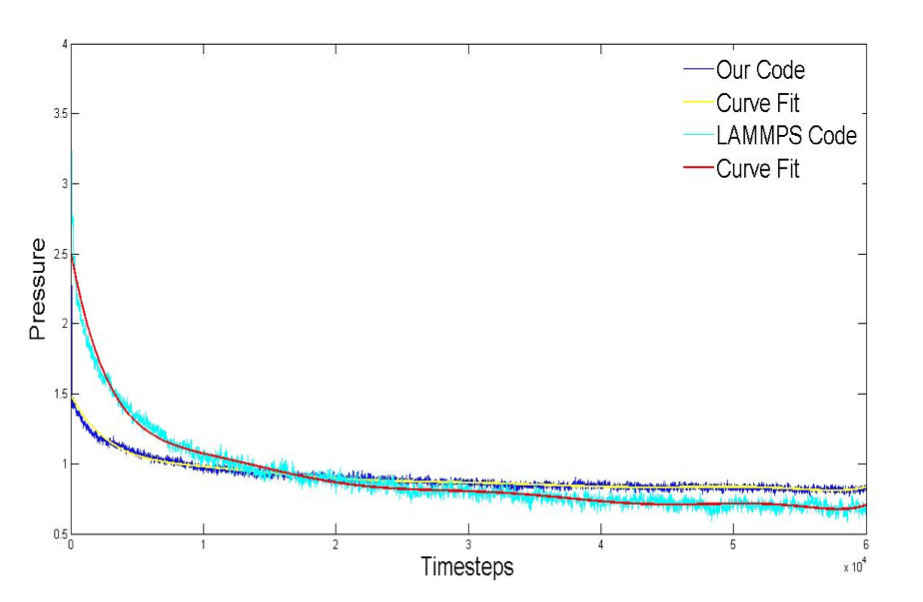
\includegraphics[width=6in]{figures/pressure.png}
\caption{Pressure over simulation run averaged across 10 trials.}
\label{fig:valpress}
\end{center}
\end{figure}

\begin{figure}
\begin{center}
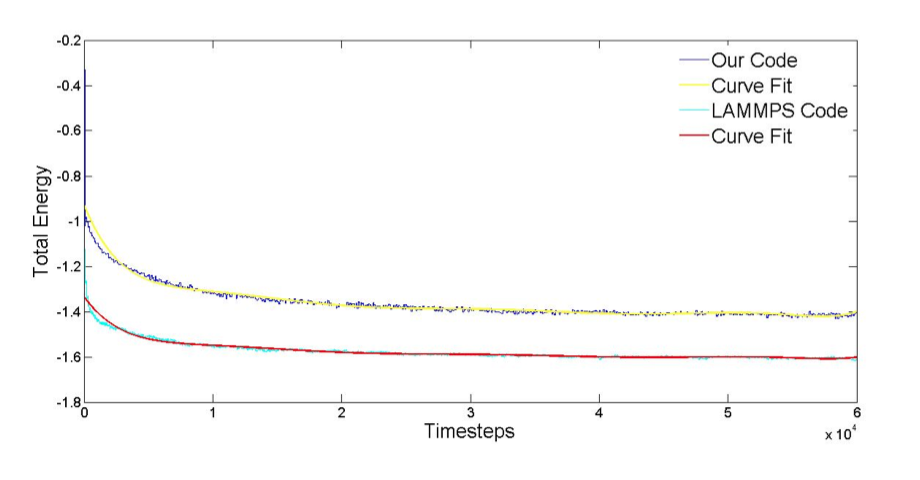
\includegraphics[width=6in]{figures/energy.png}
\caption{Total energy over simulation run averaged across 10 trials.}
\label{fig:valtot}
\end{center}
\end{figure}

\begin{figure}
\begin{center}
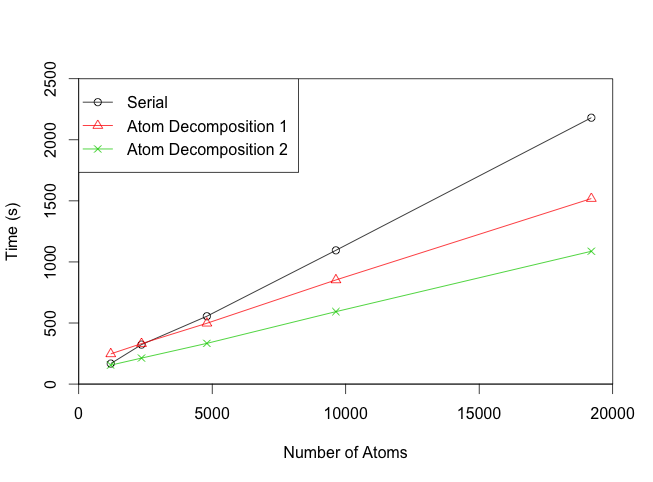
\includegraphics[width=6in]{figures/scaling.png}
\caption{Weak scaling performance of the three implementations.}
\label{fig:weakscale}
\end{center}
\end{figure}


\end{document}